\documentclass[a4paper,12pt]{article}

% -------------------------------------------------
% Pakiety
% -------------------------------------------------
\usepackage[utf8]{inputenc}
\usepackage[T1]{fontenc}
\usepackage{lmodern}
\usepackage[polish]{babel}
\usepackage{geometry}
\usepackage{graphicx}
\usepackage{float}
\usepackage{listings}
\usepackage{xcolor}
\usepackage{hyperref}
\usepackage{longtable}
\usepackage{titlesec}
\usepackage{tabularx}   % dla automatycznego zawijania tekstu i obliczania szerokości
\usepackage{booktabs}   % dla profesjonalnych linii w tabeli
\usepackage{caption}    % dla ładnego podpisu tabeli

\usepackage{hyperref}

\usepackage{dirtree}

\graphicspath{{images/}}
\geometry{margin=2.5cm}

% -------------------------------------------------
% Konfiguracja kodu źródłowego
% -------------------------------------------------
\usepackage{listings}
\usepackage{xcolor}

% Definicja kolorów dla Pythona
\definecolor{codegreen}{rgb}{0,0.6,0}
\definecolor{codegray}{rgb}{0.5,0.5,0.5}
\definecolor{codepurple}{rgb}{0.58,0,0.82}
\definecolor{backcolour}{rgb}{0.95,0.95,0.95} % Twoje dotychczasowe jasnoszare tło

\lstset{
    language=Python,
    extendedchars=true,
    keepspaces=true,
    backgroundcolor=\color{backcolour},   
    commentstyle=\color{codegreen},
    keywordstyle=\color{blue},          % Słowa kluczowe (if, and, or, is, not) będą niebieskie
    numberstyle=\scriptsize\color{codegray}, % Nieco większa czcionka niż \tiny
    stringstyle=\color{codepurple},
    basicstyle=\ttfamily\small,
    breakatwhitespace=false,         
    breaklines=true,                 
    keepspaces=true,                 
    numbers=left,                   % Doda numery linii (usuń tę linię, jeśli wolisz bez numerów)
    numbersep=7pt,                  
    showstringspaces=false,
    tabsize=4
}

% -------------------------------------------------
% Dane dokumentu
% -------------------------------------------------
\title{Dokumentacja Projektu}
\author{Jakub Kuczkowski}
\date{\today}

% -------------------------------------------------
% Początek dokumentu
% -------------------------------------------------
\begin{document}

\maketitle

\tableofcontents
\newpage

% =================================================
% WSTĘP
% =================================================

\section{Wstęp}

\noindent Projekt został przygotowany w celu stworzenia uniwersalnego, cyfrowego systemu do precyzyjnego mierzenia i analizowania ruchu ciał w czasie rzeczywistym. Głównym założeniem było zastąpienie niedokładnych, ręcznych metod pomiarowych (takich jak tradycyjne stopery) nowoczesnym układem automatycznym, który eliminuje błędy ludzkiego refleksu i dostarcza precyzyjne dane laboratoryjne.

\vspace{0.3cm}
\noindent Zastosowanie projektu obejmuje przede wszystkim szkolne i akademickie laboratoria fizyczne. System pozwala na dokładne badanie kinematyki i dynamiki różnych zjawisk – od analizy ruchu jednostajnie przyspieszonego wózków na równi pochyłej, aż po badanie okresu i amplitudy drgań poziomych oscylatorów harmonicznych (ciężarków na sprężynach). Dzięki funkcji nakładania i ręcznego przesuwania wykresów, oprogramowanie umożliwia uczniom bezpośrednie i czytelne porównywanie parametrów ruchu dla różnych konfiguracji sprzętowych (np. zmiana kąta nachylenia toru, zmiana masy ciała lub sztywności sprężyny).

\vspace{0.3cm}
\noindent Środowisko pracy systemu składa się ze stanowiska sprzętowego oraz komputera PC. Część sprzętowa to miniaturowy czujnik laserowy LIDAR (działający w technologii Time-of-Flight) oraz fizyczny przycisk wyzwalający, które są połączone z mikrokontrolerem Arduino. Część programowa to aplikacja analityczna z graficznym interfejsem użytkownika, uruchamiana na komputerze w systemie operacyjnym Linux lub Windows. Komunikacja między komputerem a Arduino odbywa się za pomocą standardowego kabla USB przez port szeregowy (UART) z prędkością transmisji \texttt{115200 bodów}.

\newpage
\subsection*{Struktura projektu}

Repozytorium projektu zostało zorganizowane w logiczną strukturę modułową, która precyzyjnie rozdziela warstwę sprzętową (kod mikrokontrolera), oprogramowanie komputerowe (aplikację monitorującą w Pythonie) oraz kompletną dokumentację. Poniżej przedstawiono szczegółowy opis roli i zawartości poszczególnych plików wchodzących w skład systemu.

\begin{itemize}
    \item \lstinline[language=Python]|LICENSE| -- Plik z licencją określającą zasady korzystania z kodu.
    \item \texttt{README.md} -- Instrukcja startowa w formacie tekstowym. Opisuje, jak szybko włączyć program i czego potrzeba do jego uruchomienia.
    \item \textbf{Katalog \texttt{arduino/}} -- Zawiera kod dla płytki Arduino, która steruje laserem i przyciskiem.
    \begin{itemize}
        \item \texttt{doc/} -- Folder na notatki, schematy kabli i opisy techniczne sprzętu.
        \item \texttt{lib/TFLidar/} -- Gotowa biblioteka (sterownik) do obsługi czujnika laserowego. Zawiera pliki kodu (\texttt{TFLidar.cpp}, \texttt{TFLidar.h}) oraz przykład (\texttt{lidar-basic-read.ino}), który pozwala sprawdzić, czy sam laser działa.
        \item \texttt{src/main.cpp} -- Główny program dla mikrokontrolera Arduino. Odpowiada za bezblokadowy odczyt odległości z czujnika LIDAR na pełnej prędkości oraz sprzętową filtrację styków fizycznego przycisku (\textit{debouncing}) na bazie czasu systemowego, bez użycia wstrzymujących procesor funkcji opóźniających.
        
        \vspace{0.3cm}
        \noindent \textbf{UWAGA:} Zarówno ta biblioteka, jak i plik \texttt{main.cpp} muszą zostać wgrane na płytkę Arduino za każdym razem, gdy zmienisz ich zawartość lub gdy podłączysz zupełnie nową płytkę. Więcej o tym, jak to zrobić krok po kroku, poszukaj na oficjalnej stronie internetowej Arduino w sekcji dokumentacji lub w podstawowych poradnikach dla początkujących użytkowników Arduino IDE.
    \end{itemize}
    
    \item \textbf{Katalog \texttt{instructions/}} -- Folder z dokumentami i instrukcją dla użytkownika.
    \begin{itemize}
        \item \texttt{dokumentacja\_projektu.tex} -- Plik źródłowy tego dokumentu w systemie \LaTeX.
        \item \texttt{dokumentacja\_projektu.pdf} -- Gotowa do wydruku instrukcja w formacie PDF.
        \item \texttt{images/} -- Folder na zdjęcia i zrzuty ekranu z programu, które widać w instrukcji.
    \end{itemize}

    \item \textbf{Katalog \texttt{python/}} -- Zawiera programy na komputer, które odbierają dane, uśredniają je i rysują wykres.
    \begin{itemize}
        \item \texttt{distance\_monitor.py} -- Podstawowa wersja programu monitorującego z graficznym interfejsem użytkownika (GUI). 
        \item \texttt{distance\_monitor\_with\_button.py} -- Główna i pełna wersja programu.
        \item \texttt{serial\_dev.py} -- Program testowy. Udaje podłączone Arduino i wysyła sztuczne dane, co pozwala testować wygląd wykresu na komputerze bez podłączania prawdziwego sprzętu.
    \end{itemize}
\end{itemize}

\newpage
\begin{figure}[ht]
\centering
\begin{minipage}{0.6\textwidth} % Keeps the tree neatly aligned
\dirtree{%
.1 InclinedPlane.
.2 LICENSE.
.2 README.md.
.2 arduino.
.3 doc.
.3 lib.
.4 TFLidar.
.5 README.md.
.5 example.
.6 lidar-basic-read.
.7 lidar-basic-read.ino.
.5 keywords.txt.
.5 library.properties.
.5 src.
.6 TFLidar.cpp.
.6 TFLidar.h.
.3 src.
.4 main.cpp.
.2 instructions.
.3 dokumentacja\_projektu.tex.
.3 dokumentacja\_projektu.pdf.
.3 images.
.4 \dots.
.2 python.
.3 distance\_monitor.py.
.3 distance\_monitor\_with\_button.py.
.3 serial\_dev.py.
.3 serial\_dev\_harmonics.py.
}
\end{minipage}
\captionsetup{justification=centering}
\caption{Struktura projektu.\\ \textbf{Repozytorium GitHub:} \url{https://github.com/Z1moRG/InclinedPlane}}
\end{figure}

% =================================================
% CZĘŚĆ 1
% =================================================
\newpage
\section{Obsługa programu}

\subsection{Metodyka wyzwalania pomiarów i kontroli czasu eksperymentu}

\noindent Podstawą poprawnego przeprowadzenia każdego doświadczenia z zakresu kinematyki lub dynamiki jest precyzyjna kontrola momentu rozpoczęcia oraz zakończenia rejestracji danych. W klasycznych laboratoriach fizycznych zjawisko asynchroniczności (opóźnienia między ręcznym włączeniem stopera a fizycznym puszczeniem badanego ciała) jest głównym źródłem błędów pomiarowych i utrudnia późniejszą analizę porównawczą wykresów. Aby wyeliminować ten problem, omawiany system pomiarowy został zaprojektowany w sposób elastyczny i pozwala na wyzwalanie rejestracji danych na dwa całkowicie niezależne sposoby: programowy oraz sprzętowy.

\vspace{0.3cm}
\noindent Pierwszy sposób to wyzwalanie czysto programowe, realizowane bezpośrednio z poziomu komputera zarządzającego eksperymentem. Jest ono dedykowane do doświadczeń, w których badacz ma pełną swobodę czasową i nie musi fizycznie asystować przy samym torze pomiarowym w ułamku sekundy, w którym rusza rejestracja. Metoda ta doskonale sprawdza się w badaniach obiektów poruszających się cyklicznie, takich jak oscylatory harmoniczne, gdzie ruch trwa nieprzerwanie, a moment włączenia zapisu nie wpływa na ostateczny kształt rejestrowanej amplitudy czy okresu drgań.

\vspace{0.3cm}
\noindent Drugi sposób to wyzwalanie sprzętowe, które wykorzystuje fizyczny przycisk zaimplementowany bezpośrednio na płytce mikrokontrolera stanowiska badawczego. Podejście to całkowicie zmienia model interakcji z urządzeniem i zamienia przycisk w sprzętowy pilot zdalnego sterowania o charakterze automatycznego wyzwalacza pomiaru. Idea ta opiera się na eliminacji błędów ludzkiego refleksu w doświadczeniach ściśle dynamicznych, takich jak zjazd wózka z równi pochyłej. Użytkownik, zamiast operować myszką komputera, ręcznie blokuje wózek na szczycie toru, jednocześnie wciskając fizyczny przycisk. Wciśnięcie przycisku informuje program, że układ znajduje się w stanie uzbrojenia i oczekiwania. W ułamku sekundy, w którym użytkownik puszcza wózek i zwalnia blokadę, przycisk wysyła do komputera sygnał o zmianie stanu elektrycznego. System natychmiast i samoczynnie inicjalizuje zbieranie danych z lasera. Ponieważ moment ruszenia ciała i moment startu pomiaru są sprzętowo zsynchronizowane, wykres generuje się bez żadnych martwych faz oczekiwania, co ma fundamentalne znaczenie dla dokładności naukowej eksperymentu.

\vspace{0.3cm}
\noindent Równie istotnym filarem logiki systemu jest koncepcja dynamicznego \textit{\textbf{timeoutu}}, czyli ręcznie definiowanego czasu trwania pomiaru. W fizyce laboratoryjnej czas trwania obserwacji musi być ściśle dopasowany do dynamiki badanego zjawiska. Za długa rejestracja skutkuje zbieraniem szumu informacyjnego po zatrzymaniu się obiektu, co zniekształca skalę wykresu, z kolei czas zbyt krótki może uciąć kluczową fazę ruchu. Użytkownik przed każdym przejazdem ma możliwość elastycznego określenia długości trwania okna pomiarowego w milisekundach. Pozwala to badaczowi na strategiczne zaplanowanie doświadczenia - od ultrakrótkich, dynamicznych sesji trwających zaledwie dwie sekundy dla stromych równi pochyłych, aż po długie, kilkudziesięciosekundowe obserwacje powolnego zanikania drgań w tłumionych oscylatorach harmonicznych. Po upływie tego precyzyjnie zdefiniowanego czasu, niezależny zegar systemowy komputera bezwarunkowo przerywa pętlę pomiarową, automatycznie zamyka serię i przywraca stanowisko do stanu pełnej gotowości na kolejny etap badań.



\subsection{Uruchamianie programu}

\subsubsection{Uruchamianie części Arduino}
Aby przygotować część sprzętową do pracy, należy wykonać następujące kroki:

\begin{enumerate}
    \item Podłączyć Arduino do komputera za pomocą standardowego kabla \texttt{USB}. Komputer powinien automatycznie wykryć urządzenie i przypisać mu odpowiedni port komunikacyjny (\texttt{COM} na systemie \texttt{Windows} lub \texttt{ttyACM/ttyUSB} na systemie \texttt{Linux}).
    \item Sprawdzić poprawność podłączenia wszystkich pinów. Czujnik laserowy \texttt{LIDAR} musi mieć prawidłowo wpięte cztery przewody: zasilanie do pinu \texttt{5V}, masę do pinu \texttt{GND}, oraz kable sygnałowe (zielony i biały) odpowiednio do pinów 10 i 11 mikrokontrolera. Dodatkowo fizyczny przycisk startowy musi być połączony z pinem 4 oraz masą (\texttt{GND}). Złe połączenie lub luźne kable spowodują, że program nie odbierze danych z lasera lub nie zareaguje na puszczenie wózka.
    \item Upewnić się, czy oprogramowanie jest wgrane na płytkę. Jeśli jest to nowe \texttt{Arduino}, zawartość plików została zmieniona lub czujnik nie wysyła danych, należy otworzyć program \texttt{Arduino IDE} i ponownie wgrać program na płytkę.
\end{enumerate}

\subsubsection{Uruchamianie części systemowej}

Aplikację na komputerze można uruchomić na dwa sposoby, w zależności od przygotowania stanowiska:

\begin{itemize}
    \item Uruchomienie bezpośrednio przez plik \texttt{Python}. Wymaga to zainstalowanego środowiska \texttt{Python 3} na komputerze. Przed włączeniem programu należy upewnić się, że pobrano wszystkie wymagane biblioteki (takie jak \texttt{PySerial} do komunikacji oraz \texttt{Matplotlib} do rysowania wykresów) i środowisko jest poprawnie skonfigurowane. Program włącza się, uruchamiając główny plik \texttt{distance\_monitor\_with\_button.py}.
    \item Uruchomienie przez gotowy plik wykonywalny \texttt{EXE}. Jest to najszybsza metoda, która nie wymaga instalowania Pythona ani żadnych dodatkowych bibliotek na komputerze. Wystarczy wejść do katalogu programu i kliknąć dwukrotnie myszką na plik wykonywalny z rozszerzeniem \texttt{.exe}. Program włączy się od razu w gotowym oknie graficznym, samoczynnie przeszuka porty USB i połączy się z działającym Arduino.
\end{itemize}



\subsection{Opis interfejsu użytkownika}

Program stanowi intuicyjne, graficzne centrum laboratoryjne służące do rejestracji i analizy zjawisk kinematycznych w czasie rzeczywistym. Cała interakcja z systemem pomiarowym odbywa się za pomocą jednego, zintegrowanego okna graficznego, co eliminuje konieczność znajomości środowisk programistycznych czy obsługi konsoli tekstowej. 

\vspace{0.3cm}
\noindent Po uruchomieniu aplikacji system automatycznie przeprowadza skanowanie portów USB komputera w poszukiwaniu podłączonej płytki Arduino z czujnikiem LIDAR. Jeśli urządzenie zostanie wykryte, użytkownik od razu widzi przygotowany, czysty układ współrzędnych (Droga w funkcji Czasu) z widoczną siatką pomocniczą, etykietami osi oraz dynamicznym celownikiem pomiarowym, który w postaci czerwonego krzyża precyzyjnie podąża za kursorem myszy, ułatwiając natychmiastowy, wzrokowy odczyt parametrów z wykresu. 

\begin{figure}[H]
    \centering
    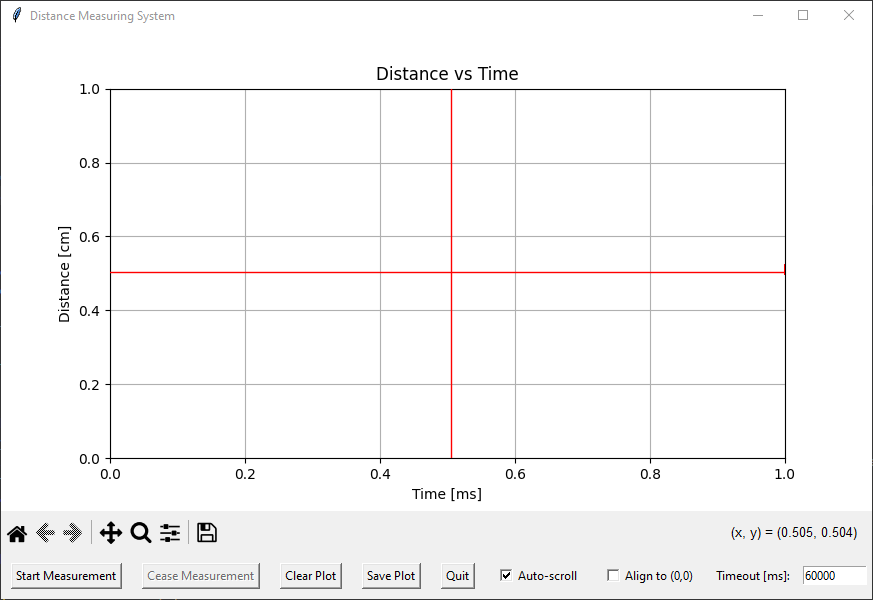
\includegraphics[width=1\textwidth]{initialLook.png}
    \captionsetup{justification=centering}
    \caption{Wygląd programu tuż po uruchomieniu.}
\end{figure}

\begin{figure}[H]
    \centering
    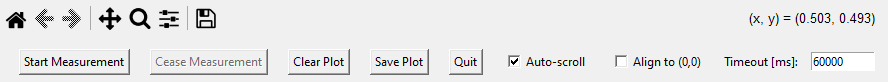
\includegraphics[width=1\textwidth]{tools.png}
    \captionsetup{justification=centering}
    \caption{Pasek narzędzi; współrzędne $(x, y)$ widoczne w prawym górnym rogu paska, to współrzędne punktu nad którym znajduje się celownik.}
\end{figure}

\vspace{0.3cm}
\noindent W celu rozpoczęcia eksperymentu (np. puszczenia wózka na równi pochyłej) użytkownik klika przycisk \textbf{\textit{Start Measurement}}. W tym momencie aplikacja automatycznie blokuje możliwość przypadkowego ponownego uruchomienia pomiaru oraz zabezpiecza strukturę wykresu przed usunięciem. Wykres ożywa - napływające z lasera dane są filtrowane i rysowane w czasie rzeczywistym. Dzięki domyślnie aktywnej funkcji \textbf{\textit{Auto-scroll}} kamera wykresu samodzielnie przesuwa się i dopasowuje granice osi tak, aby czoło rysowanej linii (najnowszy punkt) oraz cała trajektoria ruchu były idealnie widoczne na ekranie z zachowaniem czytelnego marginesu. 

\begin{figure}[H]
    \centering
    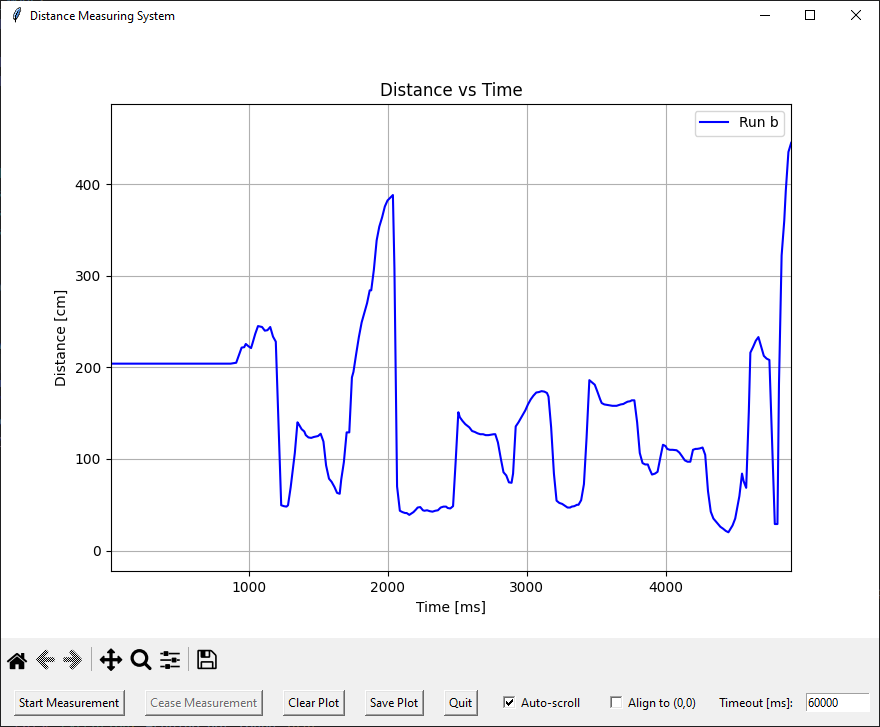
\includegraphics[width=1\textwidth]{firstRun.png}
    \captionsetup{justification=centering}
    \caption{W trakcie niektórych procesów, część przycisków jest zablokowana. Tutaj: w trakcie odczytu pomiarów nie można ponownie rozpocząć pomiaru ani wyczyścić wykresu bez wcześniejszego zatrzymania procesu.}
\end{figure}

\vspace{0.3cm}
\noindent Użytkownik ma pełną swobodę w kontrolowaniu sposobu wyświetlania danych. W dowolnym momencie może odznaczyć opcję \textbf{\textit{Auto-scroll}}, co powoduje textit{zamrożenie} pozycji kamery. Pozwala to na użycie rolki myszy do intuicyjnego przybliżania i oddalania dowolnego fragmentu wykresu (zoom) względem pozycji kursora lub skorzystanie z systemowego paska narzędzi (ruchoma rączka do przesuwania widoku, lupa). Co ważne, operacje te nie przerywają zbierania danych w tle – nowo zarejestrowane punkty są stale nanoszone na wykres, a ponowne zaznaczenie checkboxa \textbf{\textit{Auto-scroll}} natychmiast przywraca automatyczne śledzenie i kadrowanie ruchu. 

\vspace{0.3cm}
\noindent Pomiar kończy się automatycznie po upływie zdefiniowanego czasu eksperymentu (np. 10 sekund), co zapobiega powstawaniu nieskończonych linii na wykresie po zatrzymaniu wózka. Czas ten użytkownik może samodzielnie ustawić w milisekundach w dedykowanym polu tekstowym przed uruchomieniem pomiaru. Wpisana wartość jest automatycznie sprawdzana pod kątem błędów, a samo pole blokuje się po kliknięciu przycisku \textbf{\textit{Start Measurement}}, co zapobiega przypadkowym zmianom w trakcie ruchu. Użytkownik może też przerwać rejestrację w dowolnym momencie, klikając przycisk \textbf{\textit{Cease Measurement}}. Po zakończeniu pracy interfejs wraca do stanu spoczynku, a przyciski narzędziowe są ponownie odblokowywane.

\vspace{0.3cm}
\noindent Kluczową funkcjonalnością z punktu widzenia fizyki eksperymentalnej jest możliwość porównywania wielu serii pomiarowych. Każde kolejne kliknięcie \textbf{\textit{Start Measurement}} (np. po zmianie kąta nachylenia równi, właściwości oscylatora lub masy wózka) generuje na tym samym wykresie nową linię o unikalnym, automatycznie dobranym kolorze, która zostaje dopisana do dynamicznej legendy. Aby ułatwić wizualną ocenę szybkości zmian badanych wielkości dynamicznych, użytkownik może zaznaczyć opcję \textbf{\textit{Align to (0,0)}}. Powoduje to matematyczne przesunięcie nowych krzywych na wykresie w taki sposób, aby ich rzeczywiste punkty startowe nałożyły się idealnie w środku układu współrzędnych. Umożliwia to bezpośrednie i precyzyjnie porównanie nachylenia parabol lub faz oscylacji różnych serii pomiarów.

\begin{figure}[H]
    \centering
    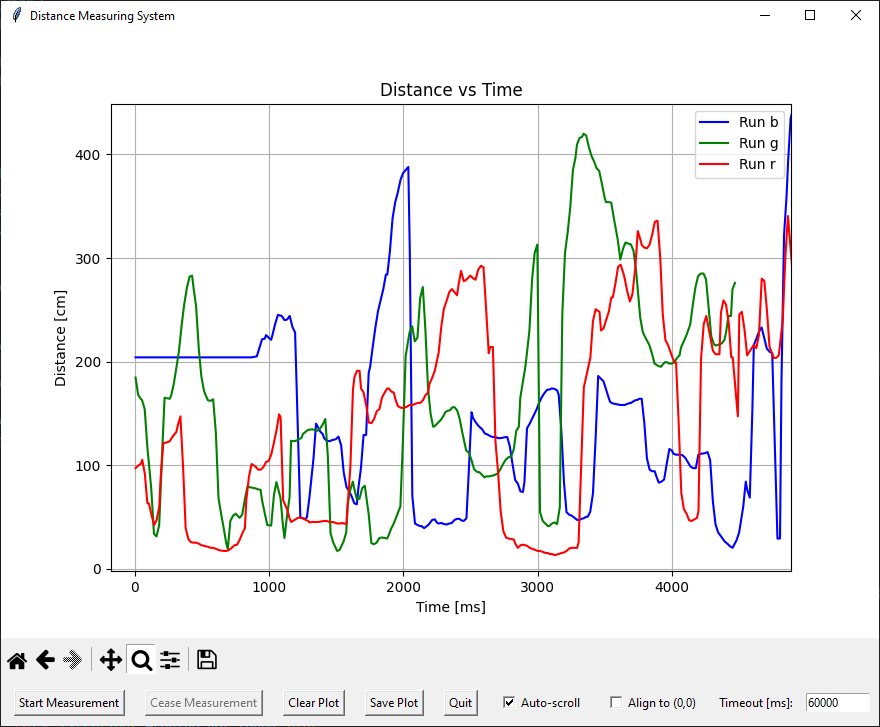
\includegraphics[width=1\textwidth]{multiploting.png}
    \captionsetup{justification=centering}
    \caption{Nałożenie wielu krzywych na jeden wykres.}
\end{figure}

\vspace{0.3cm}
\noindent Ponieważ automatyczna synchronizacja do punktu zero nakłada na siebie jedynie pierwsze zarejestrowane próbki i nie uwzględnia opóźnień wynikających z ludzkiej reakcji (np. zwolnienia wózka lub wahadła ułamek sekundy po starcie stopera), program oferuje zaawansowaną funkcję manualnej korekty geometrii wykresów za pomocą techniki przeciągnij i upuść. Po zakończeniu zbierania danych użytkownik może kliknąć lewym przyciskiem myszy bezpośrednio na wybraną linię trajektorii. Wybrana seria zostaje optycznie pogrubiona, a trzymanie wciśniętego lewego przycisku pozwala na jej płynne przesuwanie w płaszczyźnie poziomej (oś czasu) oraz pionowej (oś odległości). W trakcie tego ruchu legenda wykresu dynamicznie przekształca się w aktywny wskaźnik pomiarowy, wyświetlając w czasie rzeczywistym aktualne przesunięcie czasowe w milisekundach oraz przestrzenne w centymetrach. Pozwala to na idealne, ręczne zsynchronizowanie rzeczywistych momentów rozpoczęcia ruchu dla wszystkich serii. Po dopasowaniu wykresów, kliknięcie lewym przyciskiem myszy w dowolne puste tło układu współrzędnych powoduje bezpieczne odznaczenie linii i przywrócenie jej standardowej grubości.

\begin{figure}[H]
    \centering
    \includegraphics[width=1\textwidth]{moveit.png}
    \captionsetup{justification=centering}
    \caption{W wyniku przesunięcia krzywej legenda zmienia się (patrz prawy górny róg) uwzględniając przesunięcie w osi czasu oraz osi odległości.}
\end{figure}

\vspace{0.3cm}
\noindent Po zakończeniu serii doświadczeń i pełnej synchronizacji krzywych, użytkownik może skorzystać z przycisku \textbf{\textit{Save Plot}}, który otwiera systemowe okno menedżera plików, pozwalając na zapisanie wygenerowanego wykresu jako pliku graficznego (PNG lub JPG) do późniejszego wykorzystania w sprawozdaniu. Kliknięcie przycisku \textbf{\textit{Clear Plot}} całkowicie czyści obszar roboczy z linii, wskaźników przesunięć i legendy, przywracając domyślną skalę i resetując kolejkę kolorów przed nową serią badawczą, natomiast przycisk \textbf{\textit{Quit}} bezpiecznie zamyka połączenie z czujnikiem i wyłącza aplikację.



\subsection{Opis błędów oraz rozwiązania}

W trakcie używania systemu pomiarowego mogą pojawić się problemy techniczne wynikające z błędów połączenia sprzętowego lub nieprawidłowego wpisania parametrów w oknie programu. Poniżej znajduje się lista najczęstszych komunikatów awaryjnych, które aplikacja obsługuje, wraz z prostą instrukcją, jak naprawić daną usterkę.

\begin{enumerate}
    \item \textbf{Komunikat: \texttt{"No serial ports detected"} lub \texttt{"Arduino not found"} (Wyjątek \textit{SerialException})}
    \begin{description}
        \item[Kiedy występuje:] Błąd pojawia się natychmiast po uruchomieniu aplikacji systemowej, jeśli program nie potrafi znaleźć żadnego aktywnego urządzenia na magistrali USB.
        \item[Przyczyna:] Kabel USB od Arduino jest odłączony od komputera, port USB w komputerze jest uszkodzony, płytka nie ma zasilania lub w systemie operacyjnym brakuje odpowiednich sterowników (częsty problem w przypadku klonów Arduino z chipem CH340).
        \item[Rozwiązanie:] \
        \begin{itemize}
            \item Odłącz i podłącz ponownie kabel USB do innego portu w komputerze.
            \item Upewnij się, że na płytce Arduino świeci się dioda zasilania (ON).
            \item Zainstaluj sterowniki do układu CH340, jeśli komputer w ogóle nie widzi urządzenia.
            \item Jeśli pracujesz na systemie Linux (np. Ubuntu), upewnij się, że masz uprawnienia do czytania portu szeregowego (komenda \texttt{sudo usermod -a -G dialout \$USER} i ponowne zalogowanie).
        \end{itemize}
    \end{description}

    \item \textbf{Komunikat: \texttt{"Wprowadź poprawną, dodatnią liczbę milisekund!"} (Wyjątek \textit{ValueError} w polu Timeout)}
    \begin{description}
        \item[Kiedy występuje:] Błąd pojawia się po kliknięciu przycisku \textbf{\textit{Start Measurement}}, jeśli użytkownik zmodyfikował pole tekstowe czasu pomiaru.
        \item[Przyczyna:] W pole \textbf{\textit{Timeout [ms]}} wpisano tekst zamiast liczb (np. \texttt{dziesięć sekund}), pole pozostawiono całkowicie puste lub wpisano wartość mniejszą bądź równą zero (np. \texttt{-5000}).
        \item[Rozwiązanie:] Kliknij przycisk zamknięcia błędu, wyczyść pole tekstowe czasu i wpisz poprawną liczbę całkowitą określającą czas eksperymentu w milisekundach (np. \texttt{10000} dla 10 sekund lub \texttt{5000} dla 5 sekund). Program automatycznie odrzuci spacje i znaki niedrukowalne.
    \end{description}

    \item \textbf{Wykres zawiesza się na komunikacie: \texttt{"Waiting for data..."} i nie rysuje linii}
    \begin{description}
        \item[Kiedy występuje:] Program uruchamia się poprawnie, port szeregowy zostaje otwarty, ale po kliknięciu przycisku startu lub zwolnieniu przycisku na równi wykres nie rusza.
        \item[Przyczyna:] Brak fizycznej komunikacji między czujnikiem LIDAR a Arduino (błędne podłączenie pinów) lub niepoprawny format danych. Program uruchomił pętlę, ale funkcja filtrująca odrzuca puste ramki lub urwane teksty (np. \texttt{,9}), czekając na pierwszy poprawny pakiet.
        \item[Rozwiązanie:] \
        \begin{itemize}
            \item Sprawdź, czy zielony i biały przewód lasera nie poluzowały się w pinach 10 i 11.
            \item Upewnij się, że czujnik nie jest niczym zasłonięty w odległości mniejszej niż 2~cm (strefa martwa).
            \item Zresetuj całe urządzenie poprzez odłączenie i ponowne podłączenie kabla USB, a następnie wyczyść wykres przyciskiem \textit{Clear Plot} i ponów próbę.
        \end{itemize}
    \end{description}

    \item \textbf{Komunikat w konsoli: \texttt{"Odrzucono anomalny dystans / Pominięto uszkodzone dane"}}
    \begin{description}
        \item[Kiedy występuje:] W trakcie trwania pomiaru lub na samym jego starcie, w oknie konsoli tekstowej pojawiają się pojedyncze ostrzeżenia.
        \item[Przyczyna:] Chwilowe zakłócenia elektromagnetyczne na kablu USB (błędy bitowe w transmisji) lub ucieczka wózka z toru optycznego lasera (odbicie wiązki od ściany laboratorium powyżej X metrów).
        \item[Rozwiązanie:] Te komunikaty są informacją o prawidłowym działaniu filtrów aplikacji. Program automatycznie wychwytuje te błędy, wyrzuca je do kosza i nie pozwala im zepsuć wykresu ani zawiesić systemu. Nie musisz nic robić, o ile wykres rysuje się dalej. Jeśli anomalii jest za dużo, popraw stabilność toru wózka i upewnij się, że kable nie leżą obok źródeł silnych zakłóceń (np. zasilaczy sieciowych).
    \end{description}
\end{enumerate}



\newpage
% =================================================
% CZĘŚĆ 2
% =================================================

\section{Zaimplementowana logika systemu}

% -------------------------------------------------
% Logika agregacji danych
% -------------------------------------------------

\subsection{Logika agregacji danych}

\subsubsection*{Logiczne i Fizyczne Podstawy Algorytmu Agregacji}
Głównym zadaniem tego algorytmu jest inteligentna redukcja i uśrednianie danych w locie. Aby zrozumieć potrzebę jego zastosowania, musimy spojrzeć na rzeczywistość fizyczną eksperymentu.
Czujnik laserowy (LIDAR) mierzy odległość z ogromną częstotliwością. Przesyła np. 200 pomiarów na sekundę. W skali mikro (milisekundowej) ruch wózka na równi pochyłej nie jest idealnie gładki. Mamy styczność z drganiami mechanicznymi, mikroskopijnymi nierównościami powierzchni, a sam czujnik ma swoją cyfrową niedoskładność (szum), przez co odczyty mogą nieznacznie \textit{skakać} w górę i w dół o milimetry.
Gdybyśmy wrzucili te surowe dane bezpośrednio na wykres, otrzymalibyśmy grubą, \textit{poszarpaną} linię, z której trudno odczytać dokładny kształt krzywej kinematycznej. Algorytm agregacji działa jak filtr wygładzający, który porządkuje te dane w logiczne pakiety.

\begin{lstlisting}[language=Python]
AGGR = 10
def aggregate_data(times, distances):
    if not times:
        return [], []

    aggregated_times = []
    aggregated_distances = []

    current_time = times[0]
    sum_distance = 0
    count = 0

    for t, d in zip(times, distances):
        if t - current_time <= AGGR:
            sum_distance += d
            count += 1
        else:
            aggregated_times.append(current_time + AGGR // 2)
            aggregated_distances.append(sum_distance / count)

            current_time = t
            sum_distance = d
            count = 1

    aggregated_times.append(current_time + AGGR // 2)
    aggregated_distances.append(sum_distance / count)

    return aggregated_times, aggregated_distances
\end{lstlisting}

\subsubsection*{Koncepcja \textit{Koszyków Czasowych} (Time Slotting)}
Wyobraź sobie, że oś czasu eksperymentu dzielimy na równe odcinki (okienka) o szerokości zdefiniowanej przez stałą AGGR (np. 10 milisekund). Algorytm traktuje te okienka jak fizyczne koszyki.

\vspace{0.3cm}
\noindent Gdy rozpoczyna się pomiar, algorytm otwiera pierwszy koszyk na punkcie startowym (np. $t = 12{ ms}$).
Przez następne 10 milisekund (czyli dla wszystkich danych, które napłyną do momentu $t = 22{ ms}$), algorytm nie rysuje niczego na wykresie. Zamiast tego wrzuca wszystkie odczyty odległości do tego jednego koszyka, sumuje je i liczy, ile ich wpadło.
W ten sposób zbiera grupę reprezentantów dla małego wycinka czasu.

\subsubsection*{Logika Podejmowania Decyzji (Granica Koszyka)}
Algorytm analizuje każdą nadchodzącą paczkę danych i zadaje sobie pytanie retoryczne: \textit{Czy ten punkt nadal mieści się w moim obecnym koszyku?}

\begin{enumerate}
    \item Odpowiedź: TAK $\rightarrow$ Punkt jest akumulowany. Zwiększamy łączną sumę odległości i licznik próbek.
    \item Odpowiedź: NIE $\rightarrow$ Nadchodzi moment zwrotny. Ten punkt (który właśnie przekroczył granicę, np. ma czas $23{ ms}$) staje się sygnałem do zamknięcia starego koszyka.
\end{enumerate}

\noindent W tym momencie algorytm wykonuje kluczową operację matematyczno-fizyczną: zamienia całą grupę punktów z koszyka w jeden, idealny, uśredniony punkt reprezentacyjny.

\subsubsection*{Dlaczego Środek Okna? (Logika współrzędnej czasu \texorpdfstring{$X$}{X})}
Gdy koszyk jest zamykany, algorytm musi zdecydować, w którym miejscu na osi czasu ($X$) postawić punkt reprezentacyjny.

\begin{itemize}
    \item Mógłby wybrać czas pierwszego punktu z koszyka.
    \item Mógłby wybrać czas ostatniego punktu z koszyka.
    \item Wybiera środek geometryczny okna $(current\_time + AGGR // 2)$.
\end{itemize}

\noindent Dlaczego to logiczne z punktu widzenia fizyki? Ponieważ czujnik wysyła dane asynchronicznie. W jednym oknie 10-milisekundowym punkty mogą zgrupować się na początku, a w innym na końcu. Przypisanie uśrednionej odległości do idealnego środka przedziału czasowego gwarantuje, że punkty na wykresie będą rozłożone w idealnie równych odstępach czasu (np. co 10 ms). Zapobiega to zniekształceniom kształtu paraboli (ruchu przyspieszonego), które mogłyby sfałszować obliczenia prędkości.

\subsubsection*{Tłumienie Szumu (Logika współrzędnej odległości \texorpdfstring{$Y$}{Y})}
Współrzędna odległości ($Y$) punktu reprezentacyjnego to średnia arytmetyczna wszystkich odczytów z koszyka ($\bar{d} = \frac{\Sigma d}{n}$).

\begin{itemize}
    \item Fizyczny sens: Jeśli w ciągu tych 10 milisekund czujnik podał wartości: $50.1{ cm}$, $49.9{ cm}$, $50.0{ cm}$, $50.2{ cm}$ oraz jeden zaszumiony skok $51.0{ cm}$, to wyliczona średnia wyniesie około $50.24{ cm}$.
    \item Wpływ chwilowego, pojedynczego błędu (szumu) został drastycznie osłabiony przez pozostałe, stabilne pomiary. Wykres staje się gładką, ciągłą linią o wysokiej jakości estetycznej i naukowej.
\end{itemize}

\subsubsection*{Logika \textit{Domykania} (Ostatni Koszyk)}
Na samym końcu, gdy eksperyment dobiega końca lub użytkownik kliknie \textbf{\textit{Cease measurement}} pętla analizująca dane kończy pracę.
W tym momencie w ostatnim koszyku mogły zostać np. 3 punkty, które nie doczekały się oficjalnego zamknięcia (bo nie nadszedł już żaden kolejny punkt, który wybiłby algorytm do sekcji \texttt{else}).
Logika algorytmu przewiduje ten scenariusz: instrukcje umieszczone tuż przed wyjściem z funkcji wymuszają awaryjne uśrednienie i opróżnienie tego, co zostało w ostatnim koszyku. Dzięki temu żaden, nawet ostatni milimetr ruchu wózka na końcu równi pochyłej, nie zostanie zgubiony.

\subsubsection*{Podsumowanie korzyści logicznych dla fizyka:}
Algorytm ten dokonuje kompresji danych z zachowaniem praw fizyki. Zamiast obciążać komputer rysowaniem tysięcy surowych, drgających pikseli, przekształca strumień laboratoryjny w idealną matematycznie serię punktów, idealnie przygotowaną pod wyznaczanie wektora prędkości czy przyspieszenia ziemskiego.

% -------------------------------------------------
% Odrzucanie punktów anomalnych 
% -------------------------------------------------

\subsection{Logika filtrowania i odrzucania wartości anomalnych}

\noindent W trakcie przesyłania danych przez port szeregowy oraz podczas pracy lasera w warunkach laboratoryjnych mogą pojawić się zakłócenia. Objawiają się one nagłym odebraniem przez program absurdalnych wartości, na przykład czasu ujemnego lub odległości rzędu kilkunastu metrów (mimo że tor ma zaledwie dwa metry). Zakłócenia te wynikają najczęściej z przekłamań pojedynczych bitów w kablu USB (tzw. błędy transmisji) lub z chwilowej utraty celu przez laser (np. gdy wiązka odbije się od ściany lub sufitu, bo wózek lekko drgnął na boki).

\vspace{0.3cm}
\noindent Aby te fałszywe punkty (anomalie) nie zepsuły automatycznego skalowania wykresu i nie zniekształciły wyników, program stosuje dwa proste filtry bezpieczeństwa w domenie czasu i przestrzeni. Filtrowanie to odbywa się wewnątrz metody \texttt{\_read\_serial\_line}:

\begin{enumerate}
    \item \textbf{Filtr anomalii czasu:} Jeśli program obliczy czas relatywny $t$ i wyjdzie on mniejszy od zera ($t < 0$) lub dwukrotnie większy niż ustawiony czas pomiaru ($t > 2 \cdot T_{{timeout}}$), punkt jest ignorowany. Pierwszy warunek chroni przed błędami cofania się czasu, a drugi odcina szum transmisyjny. Zmienna ta jest kontrolowana w kodzie przez parametr \texttt{self.current\_timeout}.
    \item \textbf{Filtr fizycznego zasięgu lasera:} Program sprawdza, czy odczytany dystans mieści się w sztywnych granicach $[{MIN\_DISTANCE}, {MAX\_DISTANCE}]$, zdefiniowanych jako $2\,{cm}$ oraz $500\,{cm}$. Wartość poniżej $2\,{cm}$ oznacza wejście w strefę martwą czujnika, a powyżej $500\,{cm}$ to ewidentne odebranie odbicia od elementów tła laboratorium.
\end{enumerate}

\noindent Jeśli jakakolwiek próbka nie spełni tych kryteriów, funkcja odczytu zwraca wartość \texttt{None}, co dla pętli głównej jest sygnałem do pominięcia tego punktu i przejścia do kolejnej iteracji.

\vspace{0.3cm}
\noindent Poniżej przedstawiono fragment kodu z metody \texttt{\_read\_serial\_line}, który bezpośrednio odpowiada za tę logikę:

\begin{lstlisting}[language=Python]
try:
    t_raw = int(parts[0].strip())
    d = int(parts[1].strip())
    btn_state = int(parts[2].strip())
except ValueError:
    print(f"Pominieto uszkodzone dane transmisyjne: {data}")
    return None

# Jedyny filtr na tym etapie: fizyczny zakres pracy sensora LIDAR
MIN_DISTANCE = 2    # cm
MAX_DISTANCE = 300  # cm
if d < MIN_DISTANCE or d > MAX_DISTANCE:
    return None

return t_raw, d, btn_state
\end{lstlisting}

\vspace{0.3cm}
\noindent Uzupełnieniem tego mechanizmu jest centralne sprawdzenie czasu w głównej pętli pomiarowej metody \texttt{update\_plot}, zaprezentowane na poniższym listingu:
\vspace{0.3cm}

\begin{lstlisting}[language=Python]
# Obliczenie czasu relatywnego
t = t_raw - t0

# Filtr anomalii chroniacy przed rzadkimi bledami skokow rejestru
if t < 0 or t > self.current_timeout * 2.0:
    continue
\end{lstlisting}

\vspace{0.3cm}
\noindent Dzięki takiemu podziałowi ról, surowy strumień danych jest skutecznie oczyszczany przed jakimkolwiek rysowaniem. Wykres pozostaje idealnie wykadrowany na rzeczywisty ruch wózka lub oscylatora, a baza danych w tablicach \texttt{raw\_ts} oraz \texttt{raw\_ds} jest wolna od zakłóceń, co gwarantuje pełną poprawność i stabilność działania programu przy każdym kolejnym powtórzeniu eksperymentu.

\vspace{0.3cm}
\noindent \textbf{UWAGA:} Wstępne ograniczanie odległości odbywa się już na poziomie płytki Arduino w pliku \texttt{main.cpp}. Zastosowany tam warunek $if (distance < 600)$ odrzuca wszystkie odczyty powyżej 600 centymetrów (6 metrów). Jest to podyktowane fizyczną specyfikacją czujnika LIDAR, którego maksymalny zasięg stabilnej pracy wewnątrz pomieszczeń wynosi około 12 metrów, natomiast w warunkach laboratoryjnych wartości powyżej 6 metrów są traktowane jako błąd i bezużyteczny szum pomiarowy, którego nie warto przesyłać do komputera.



\newpage
% =================================================
% CZĘŚĆ 3
% =================================================

\section{Opis sprzętu oraz połączeń}

\begin{table}[htbp]
    \centering
    \label{tab:komponenty}
    \begin{tabularx}{\textwidth}{@{} l X @{}}
        \toprule
        \textbf{Komponent} & \textbf{Opis} \\
        \midrule
        Arduino Uno          & Główny mikrokontroler sterujący pracą systemu. \\
        Benewake TFmini Plus & Laserowy czujnik odległości klasy LiDAR działający w technologii ToF (Time-of-Flight). \\
        Przycisk & Opcjonalna funkcja rozpoczęcia pomiaru. \\
        Przewody połączeniowe& Elastyczne przewody sygnałowe i zasilające (raster 1,27~mm od strony czujnika). \\
        \bottomrule
    \end{tabularx}
    \caption{Zestawienie głównych komponentów systemu.}
\end{table}

\begin{figure}[H]
    \centering
    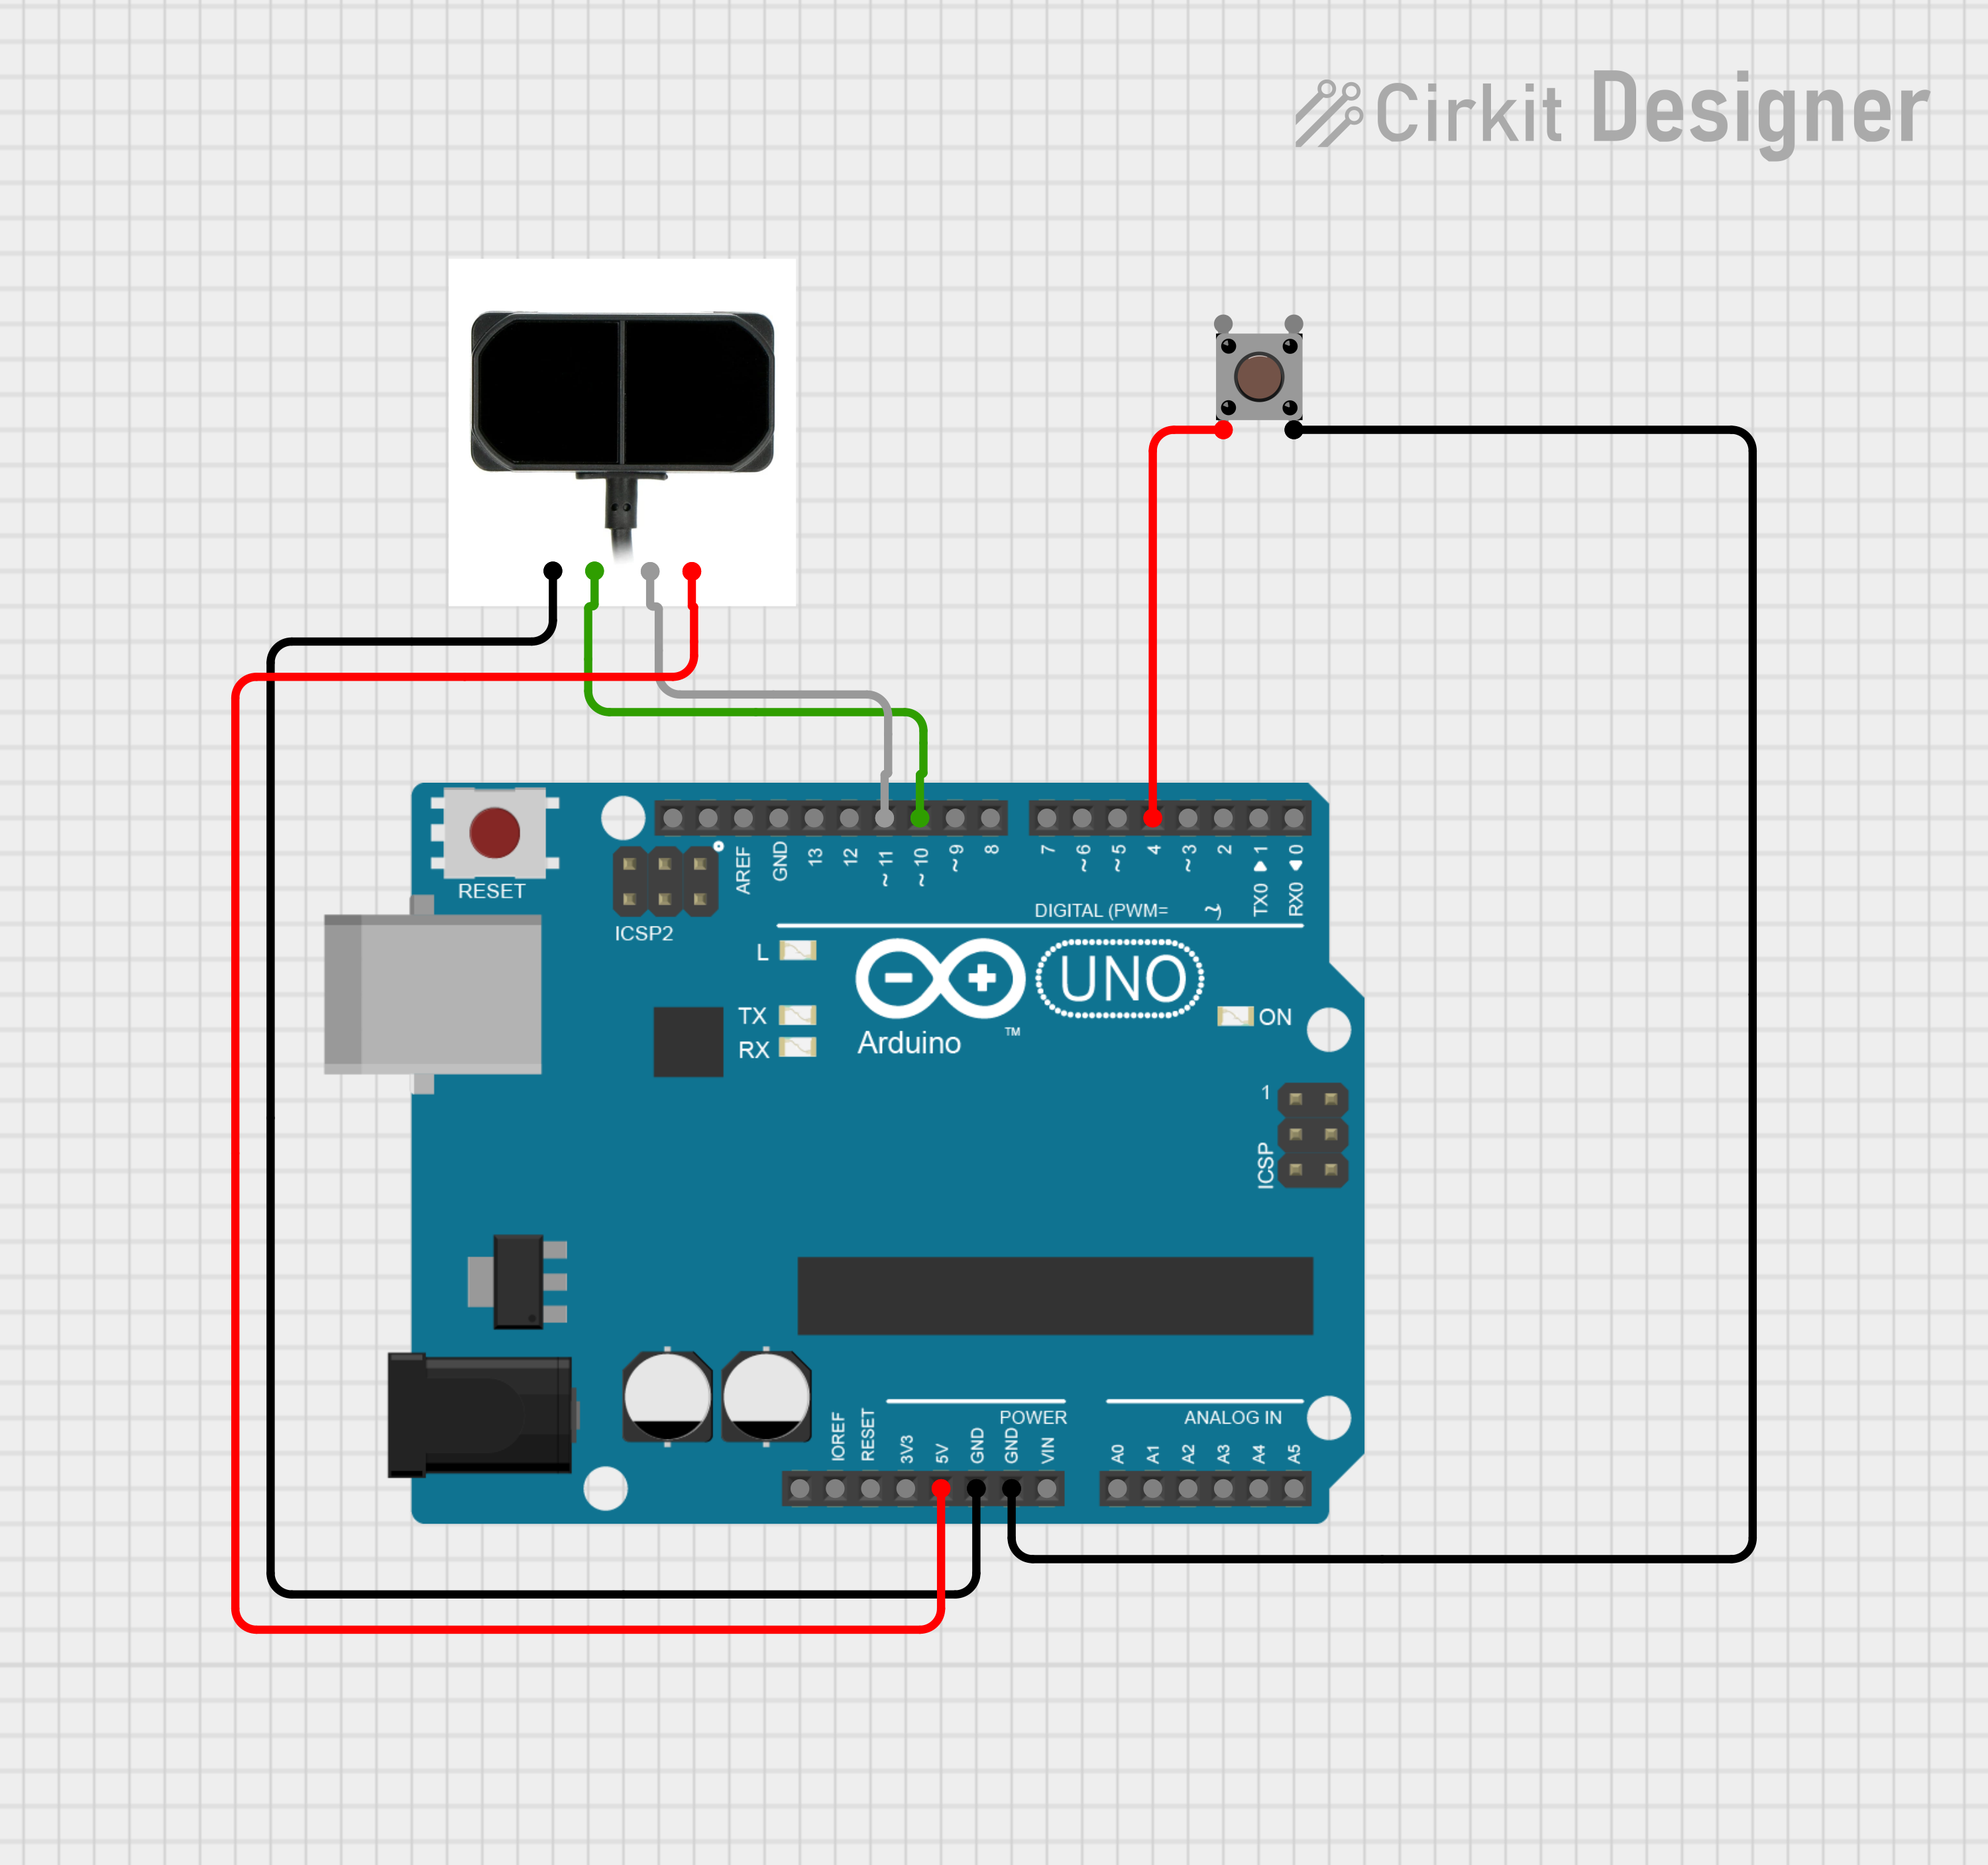
\includegraphics[width=1\textwidth]{circuit_imagep2.png}
    \caption{Schemat połączeń układu}
\end{figure}

\begin{table}[htbp]
    \centering
    \label{tab:piny_tfmini}
    \begin{tabularx}{\textwidth}{@{} l l X @{}}
        \toprule
        \textbf{Pin} & \textbf{Podłączony element} & \textbf{Opis} \\ 
        \midrule
        10 (RX) & TFmini Plus - Pin TX (Zielony) & Cyfrowa linia odbioru danych (UART). \\ 
        11 (TX) & TFmini Plus - Pin RX (Biały) & Cyfrowa linia nadawania danych (UART). \\ 
        GND     & TFmini Plus - Pin GND         & Wspólna masa (uziemienie) układu. \\ 
        5V      & TFmini Plus - Pin VCC         & Szyna zasilania sensora laserowego. \\ 
        4       & Przycisk (Styk A)             & Sygnał wejściowy (funkcja \texttt{INPUT\_PULLUP}). \\ 
        GND     & Przycisk (Styk B)             & Zwarcie pinu do masy po wciśnięciu. \\ 
        \bottomrule
    \end{tabularx}
    \caption{Opis połączeń pinów dla modułu TFmini Plus i przycisku.}
\end{table}


\subsection*{Zasilanie układu}

Układ pomiarowy zasilany jest napięciem stałym o wartości $5{V}$ ($\pm 0{,}5{V}$) dostarczanym bezpośrednio z dedykowanego pinu mikrokontrolera Arduino Uno. Maksymalny pobór prądu przez czujnik laserowy TFmini Plus wynosi $110{mA}$ przy stałej pracy pomiarowej. Stabilizacja napięcia zasilania jest kluczowa dla zachowania deklarowanej przez producenta dokładności oraz uniknięcia błędów nasycenia fotodiody przy silnym świetle odbitym.

\subsection*{Parametry techniczne}

Szczegółowe specyfikacje czujnika odległości, wyznaczone na podstawie rzeczywistych ograniczeń laboratoryjnych oraz danych producenta, zestawiono w poniższej tabeli. Kompletna specyfikacja i dokumentacja techniczna urządzenia zawarta jest w osobnym pliku: \texttt{TFminiPlus\_datasheet.pdf}.

\begin{table}[H]
    \centering
    \label{tab:parametry_tfmini}
    \begin{tabularx}{\textwidth}{@{} X l @{}}
        \toprule
        \textbf{Parametr} & \textbf{Wartość fabryczna / Zakres} \\
        \midrule
        Zakres roboczy (zasięg)           & Od $0{,}1{m}$ do $12{m}$ \\
        Dokładność pomiarowa              & $\pm 5{cm}$ (do $6{m}$), $1\%$ (powyżej $6{m}$) \\
        Częstotliwość pracy (odświeżanie) & Od $1{Hz}$ do $1000{Hz}$ (regulowana) \\
        Kąt widzenia (FOV)                 & $3{,}6^\circ$ \\
        Napięcie zasilania                & $5{V} \pm 0{,}5{V}$ \\
        Interfejsy komunikacyjne          & UART, ${I}^2{C}$ \\
        Klasa szczelności obudowy         & IP65 \\
        Masa modułu                       & $11{g}$ \\
        \bottomrule
    \end{tabularx}
    \caption{Specyfikacja techniczna i parametry robocze czujnika TFmini Plus.}
\end{table}

\newpage

% =================================================
% CZĘŚĆ 4
% =================================================

\section{Alternatywne Zastosowania Systemu Pomiarowego}

\subsection{Badanie i Porównywanie Poziomych (Pionowych) Oscylatorów Harmonicznych}

Dzięki uniwersalnej architekturze filtracji danych oraz zaawansowanym algorytmom manipulacji geometrią wykresu w czasie rzeczywistym, oprogramowanie to wykracza poza ramy badania ruchu postępowego na równi pochyłej i może być z powodzeniem stosowane w innych kluczowych działach fizyki klasycznej. Wyjątkowo wartościowym dydaktycznie i naukowo zastosowaniem systemu jest analiza porównawcza poziomych oscylatorów harmonicznych (ciężarków na sprężynach poruszających się po torze o minimalnym tarciu). W tego typu doświadczeniach kluczowym wyzwaniem metrologicznym jest precyzyjne określenie położenia równowagi jako fizycznego punktu zero oraz zsynchronizowanie fazy ruchu drgającego dla układów o różnych właściwościach fizycznych. Poniższa instrukcja krok po kroku opisuje metodologię przeprowadzenia takiego eksperymentu za pomocą przygotowanego narzędzia.

\vspace{0.3cm}
\noindent W pierwszej kolejności użytkownik musi przygotować stanowisko badawcze i uruchomić aplikację. Przed rozpoczęciem jakiejkolwiek rejestracji danych, kluczowe jest aktywowanie na panelu sterowania funkcji \textbf{\textit{Align to (0,0)}} oraz fizyczne umieszczenie ciężarka w stanie spoczynku, dokładnie w jego naturalnym położeniu równowagi. W tej pozycji siła sprężystości sprężyny oraz siła ciężkości równoważą się, a odległość mierzona przez czujnik laserowy stanowi bazę odniesienia dla całego późniejszego ruchu.

\vspace{0.3cm}
\noindent Procedurę pomiarową rozpoczyna się poprzez kliknięcie przycisku \textbf{\textit{Start Measurement}}, gdy ciało wciąż znajduje się w bezruchu w położeniu równowagi. Jest to krok o charakterze krytycznym z punktu widzenia logiki programu. Ponieważ funkcja wyrównywania pobiera absolutnie pierwszy odebrany punkt pomiarowy jako środek nowego układu współrzędnych, program natychmiast przypisuje aktualną pozycję spoczynkową jako matematyczny punkt zero w przestrzeni i czasie. Dopiero po ułamku sekundy od kliknięcia przycisku i zarejestrowaniu punktu startowego, użytkownik manualnie wychyla ciężarek z położenia równowagi o pożądaną amplitudę, po czym swobodnie puszcza oscylator.

\vspace{0.3cm}
\noindent W tym momencie na ekranie komputera zaczyna rysować się klasyczna sinusoida ruchu drgającego, odzwierciedlająca zmiany położenia ciała w funkcji czasu. Ponieważ czas i droga zaczęły być naliczane od punktu równowagi, wykres idealnie symetrycznie obrazuje wychylenia w kierunku dodatnim (od czujnika) oraz ujemnym (w stronę czujnika), co pozwala na bezpośredni odczyt amplitudy drgań bez konieczności wykonywania ręcznych obliczeń różnicowych. Po zarejestrowaniu kilku pełnych okresów drgań, użytkownik przerywa proces za pomocą przycisku \textbf{\textit{Cease Measurement}} lub pozwala programowi na automatyczne zakończenie pomiaru po upływie zdefiniowanego czasu eksperymentu.

\begin{figure}[H]
    \centering
    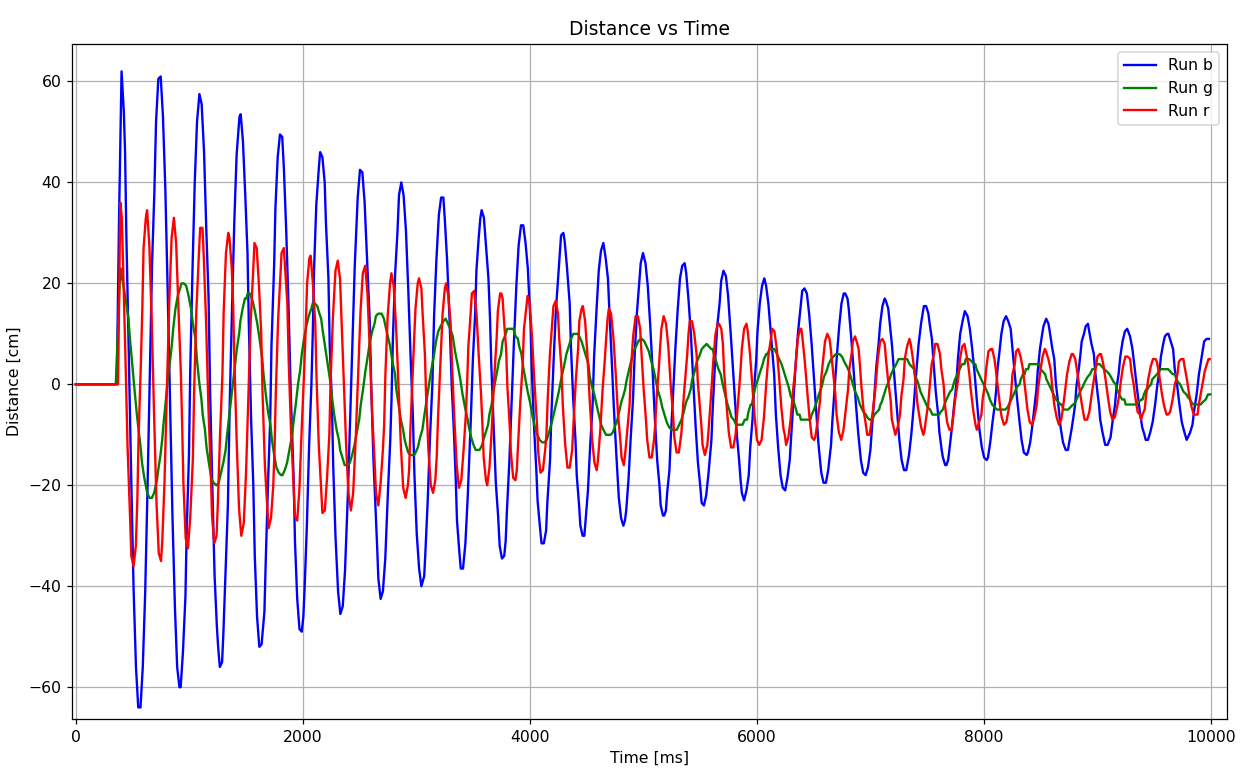
\includegraphics[width=1\textwidth]{ruchHarmoniczny.png}
    \caption{Zasymulowany ruch harmoniczny (\texttt{serial\_dev\_harmonics.py})}
\end{figure}

\vspace{0.3cm}
\noindent W celu dokonania analizy porównawczej, użytkownik – pod żadnym pozorem nie klikając przycisku \textbf{\textit{Clear Plot}} – zmienia właściwości fizyczne oscylatora, na przykład poprzez podpięcie sprężyny o innej stałej sztywności k lub zmianę masy drgającego ciężarka. Następnie powtarza dokładnie całą procedurę: ustawia nowe ciało w jego własnym położeniu równowagi, uruchamia pomiar, wychyla je o taką samą lub inną amplitudę i puszcza wolno.

\vspace{0.3cm}
\noindent Na jednym ekranie komputera pojawiają się wówczas dwa lub więcej nałożone na siebie wykresy o różnych, automatycznie dobranych kolorach. Dzięki temu, że oba wykresy zostały automatycznie wyzerowane w swoich unikalnych położeniach równowagi, użytkownik uzyskuje bezprecedensową możliwość bezpośredniego porównania parametrów dynamicznych obu układów. Może natychmiastowo ocenić wzrokowo różnicę w okresie i częstotliwości drgań dla sprężyn o różnej sztywności oraz przeanalizować stopień tłumienia drgań w czasie. Ewentualne przesunięcia fazowe wynikające z niesynchronicznego puszczenia ciężarków przez człowieka można w ułamku sekundy skorygować manualnie za pomocą funkcji chwytania linii lewym przyciskiem myszy i precyzyjnego przeciągania jej wzdłuż osi czasu, co czyni to oprogramowanie niezwykle potężnym i uniwersalnym narzędziem w rękach fizyka eksperymentatora.

\newpage
% =================================================
% ZAKOŃCZENIE
% =================================================

\section{Podsumowanie}

\subsection*{Najważniejsze cechy projektu}
\noindent Najważniejsze cechy projektu to jego uniwersalność, bezbłędna stabilność działania oraz prostota obsługi. System łączy precyzję pomiaru laserowego z zaawansowanym filtrowaniem danych na żywo. Kluczowymi zaletami oprogramowania są automatyczna kompresja i wygładzanie zaszumionego sygnału, pełne zabezpieczenie przed awariami transmisji szeregowej, a także unikalna funkcja ręcznego przesunięcia i nakładania gotowych linii na wykresie za pomocą myszki.

\subsection*{Osiągnięte rezultaty}
\noindent Osiągnięte rezultaty to stworzenie w pełni sprawnego, bezbłędnie działającego stanowiska laboratoryjnego. Udało się całkowicie wyeliminować problem zawieszania programu przy starcie oraz błędy ujemnego czasu generowane przez zapchane bufory sprzętowe Arduino i błędy ludzkiego refleksu. Urządzenie z pełną dokładnością rejestruje trajektorię ruchu ciał w czasie rzeczywistym i pozwala na bezpośrednie, wzrokowe porównywanie parametrów dynamicznych różnych doświadczeń, co potwierdziły testy z wózkiem na równi oraz oscylatorem harmonicznym.

\subsection*{Możliwe kierunki rozwoju}
\noindent Możliwe kierunki rozwoju projektu obejmują przede wszystkim dodanie funkcji automatycznego dopasowywania krzywej (regresji kwadratowej) do wyznaczania przyspieszenia oraz numerycznego różniczkowania drogi w celu rysowania wykresów prędkości i przyspieszenia w dodatkowych zakładkach. Warto również rozważyć dodanie modułu automatycznego zapisu wyników do plików CSV oraz implementację bezprzewodowej transmisji danych przez moduł Bluetooth, co całkowicie uwolniłoby stanowisko pomiarowe od kabli USB.


% =================================================
% BIBLIOGRAFIA
% =================================================

\section*{Repozytorium GitHub}
\addcontentsline{toc}{section}{Informacje o repozytorium} 

Wszelkie kody źródłowe zostały zarchiwizowane i udostępnione publicznie na licencji MIT. 

\begin{quote}
    \textbf{Adres URL:} \url{https://github.com/Z1moRG/InclinedPlane}
\end{quote}


\end{document}
```
